\documentclass[12pt]{article}
\usepackage[utf8]{inputenc}
\usepackage[T1]{fontenc}
\usepackage[letterpaper,margin=0.75in]{geometry}
\renewcommand{\rmdefault}{ptm}
\usepackage[numbers]{natbib}
\usepackage[french]{babel}
\usepackage{hyperref}
\usepackage{graphicx}

\title{Projet - Agent intelligent pour le jeu Quoridor}
\author{
  Team : Cazou\\
  Virgile Retault : 2164296\\
  Sebastien Foucher : 2162248
}

\vspace{-5ex}

\begin{document}

\maketitle

\section*{Méthodologie}

Nous avons implémenté un agent utilisant l'algorithme minimax avec alphabeta pruning que nous avons amélioré avec diverses optimisations.

Tout d'abord nous avons programmé un décorateur timeit pour évaluer statistiquement le temps d'exécution de chaque fonction et nous avons remarqué que le temps d'exécution de la fonction get\_actions était très lente à cause d'un nombre élevé d'appels à get\_shortest\_path qui est un algorithme A*. Cette fonction est appelée pour chaque possibilité de nouveau mur pour vérifier que le mur est valide et ne bloque pas le chemin du joueur. Cependant on peut remarquer qu'un mur ne peut bloquer le chemin d'un joueur que si celui-ci est posé a côté d'un mur déjà existant. Nous avons donc réimplémenté la méthode is\_wall\_possible\_here de la classe Board pour ne lancer A* que dans le cas où c'est vraiment nécessaire. Cela permet de diviser le temps d'exécution par 18. 

Nous avons utilisé une heuristique simple pour l'algorithme minimax qui consiste à faire la différence entre la distance jusqu'à la victoire de l'adversaire et cette même distance pour notre joueur. Il s'agit de minimiser notre chemin en maximisant celui de l'adversaire. Un coefficient de 1.1 est appliqué sur le chemin de l'adversaire pour favoriser les coups bloquants celui-ci pour éviter les cas dans lesquels placer un mur devant l'adversaire est équivalent à avancer le joueur de 1: sans cela le joueur avancerait jusqu'au bord du plateau et ne bloquerait l'adversaire que au dernier moment. Cela permet de bloquer l'adversaire plus tôt dans le cas ou l'adversaire décide d'aller tout droit vers l'opposé du plateau. 

Notre stratégie globale utilise deux algorithmes en fonction du cas. Dans le cas où notre agent est plus proche de l'arrivée que l'adversaire, nous avons décidé de simplement bouger notre pion dans le sens du chemin le plus court (algorithme glouton). Lorsque l'adversaire est plus proche de l'arrivée que notre agent, nous utilisons minimax pour chercher à le bloquer. Si le minimax conclue qu'on doit faire un mouvement de pion, le mouvement suivant le chemin le plus court est forcément utilisé pour éviter que le pion fasse des allers retours entre deux cases car il prévoit que l'adversaire va le bloquer s'il fait autre chose. 

Pour pouvoir avoir une profondeur suffisante pour minimax (3), nous ne considérons que les placement de murs jugés utiles. Nous utilisons pour cela une heuristique qui évalue l'utilité d'un mur et nous ne conservons que les 20 mouvements ayant l'heuristique la moins élevée. Cette heuristique consiste à considéré qu'un mur est plus utile s'il est proche de l'adversaire et à côté de murs déjà existants. Cela permet de favoriser les placement de murs qui vont bloquer des chemins. Pour éviter d'avoir un algorithme déterministe, l'ordre de considération des coups dans alphabeta est aléatoire. 

Après de nombreux tests nous avons trouvé qu'une profondeur maximale de 3 pour minimax avec 20 coups considérés par nœud de l'arbre permettait de jouer une partie dans le temps attribué. Les coups qui foncent vers l'arrivée dans le cas ou notre agent est plus proche que l'adversaire permettent de réduire considérablement le temps de réflexion. 

\section*{Résultats et Evolution de l'agent}

Tableau: nombre de fois qu'on gagne contre random/glouton et contre lui même sans les 20 coups avec 2 de profondeur

Bugs contre lui même?

Voici les scores obtenus avec ces différentes méthodes:
\begin{center}
  \begin{tabular}{ |c|c| }
    \hline
    Affrontement & Nombre de victoire de l'agent final \\\hline\hline
    my\_agent vs random & 10/10 \\\hline
    random vs my\_agent & 10/10 \\\hline
    my\_agent vs greedy & 10/10 \\\hline
    greedy vs my\_agent & 10/10 \\\hline

  \end{tabular}
\end{center}


\section*{Discussion}

Notre agent final est capable de faire des coups plutôt bons mais il ne permet pas de battre un humain après plusieurs parties car il est assez natif et tombe facilement dans les pièces. Cela est du au fait qu'il fonce vers la victoire lorsqu'il est plus proche et n'a ne prévoie pas suffisamment de coup à l'avance pour voir des pièges profonds. Il n'a pas d'intuition suffisante pour se bloquer lui-même pour éviter d'être bloqué plus tard par exemple. Il faudrait beaucoup plus de profondeur pour arriver à cela. 

Le plus gros problème de notre agent lors de la compétition est qu'il essayait de faire des coups valides mais considérés comme invalides par le moteur de jeu. Cela est du à un bug dans le moteur de jeu qui est expliqué dans la section suivante. Nous avons corrigé ce bug dans la réimplémentation du moteur de jeu, ce qui nous amène à considérer des coups valides selon les règles mais invalide selon le moteur de jeu officiel. Après avoir découvert ce problème lors de la compétition, nous l'avons corrigé dans la version finale en faisant une vérification avec le moteur de jeu officiel avant de tenter de jouer un coup. 

\section*{Agent malveillant}

Pendant nos expériences, nous avons découvert un bug dans le moteur de jeu et nous avons trouvé une méthode pour l'exploiter et gagner une partie contre n'importe quel agent. Cependant nous n'avons pas souhaité utiliser cette méthode lors de la compétition car elle était déloyale. 

La plupart des fonctions du moteur de jeu renvoient une exception NoPath si elles sont appelées et qu'il n'existe aucun chemin valide. Cependant, la fonction get\_shortest\_path renvoie une exception NoPath à tord dans certains cas. En effet lorsque le seul chemin possible est obstrué par un joueur, la fonction considère qu'il n'y a pas de chemin possible, alors qu'il y en aura forcément un au tour suivant car le joueur ne peut normalement pas choisir de rester sur place sans bouger.
explain except NoPath

% TODO: insérer screenshot de la construction
\begin{figure}
	\centering
	\caption{My\_player VS Greedy\_player}
	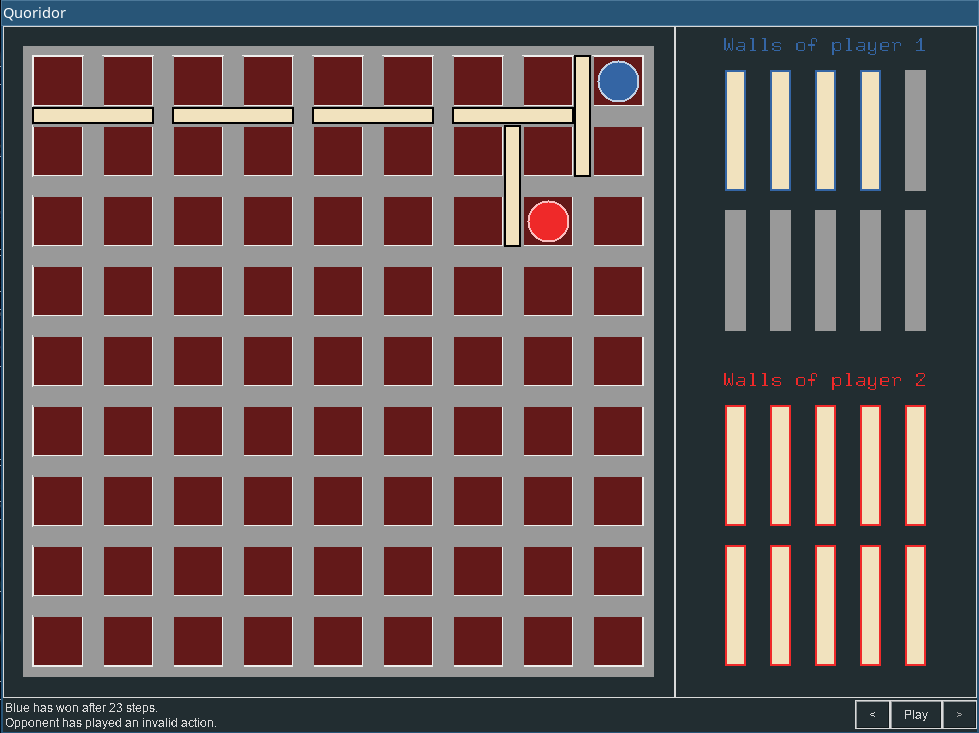
\includegraphics[width=0.75\paperwidth]{myplayer_vs_greedy.png}
    	\label{fig:arch}
\end{figure}

\begin{figure}
	\centering
	\caption{Greed\_player VS My\_player}
	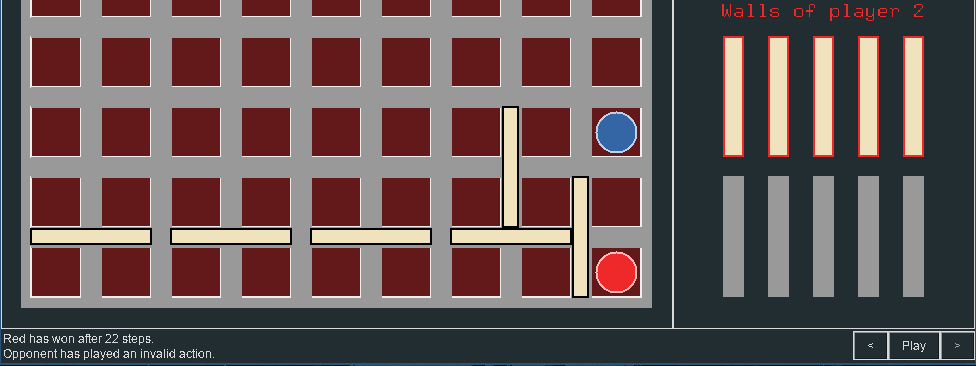
\includegraphics[width=0.75\paperwidth]{greedy_vs_myplayer.png}
	\label{fig:arch}
\end{figure}


Il est possible de construire la situation suivante pour forcer un cas où le seul chemin possible est bloqué par notre pion. Ainsi lorsque l'agent de l'adversaire fait un appel au moteur de jeu, par exemple en appelant min\_steps\_before\_victory, une erreur NoPath sera retournée faisant ainsi planter le programme de l'agent. Une contre mesure que nous avons utilisé est d'utiliser un bloc try/catch devant chaque appel au moteur de jeu pour récupérer cette exception et jouer un coup aléatoire dans ce cas. Cependant cette contre mesure ne fonctionne pas totalement car si l'adversaire décide de poser un mur, la fonction is\_wall\_possible\_here du code coté serveur va être appelée et l'adversaire va se faire renvoyer pour coup invalide. 

Le problème de cette méthode est que si l'adversaire joue des coups aléatoires sur le côté de la grille il pourrait bloquer la stratégie. Il faudrait ainsi programmer un agent qui au lieu d'essayer de gagner le jeu essaye de favoriser cette situation où le bug apparaît. Cela est beaucoup plus simple que de tenter de gagner le jeu car l'adversaire essayera lui de gagner s'il n'a pas découvert le bug. 

\end{document}

